\documentclass{mwhittaker}
\title{Bipartisan Paxos}

\usepackage{algorithmicx}
\usepackage{algorithm}
\usepackage{algpseudocode}
\usepackage{appendix}
\usepackage{mdframed}
\usepackage{mdframed}
\usepackage{multirow}
\usepackage{pervasives}
\usepackage{subcaption}
\usepackage{tikz}
\usetikzlibrary{calc}
\usetikzlibrary{positioning}
\usetikzlibrary{shapes.misc}

% Boxed invariants.
\newmdtheoremenv[
  hidealllines=true,
  innerleftmargin=8pt,%
  innerrightmargin=8pt,%
  innertopmargin=0pt,%
  innerbottommargin=8pt,%
  backgroundcolor=flatblue!20,%
  skipbelow=\baselineskip,%
  skipabove=8pt]{boxedinvariant}{Invariant}

% Misc commands.
\newcommand{\deps}[1]{\text{deps}(#1)}
\newcommand{\noop}{\text{noop}}
\newcommand{\quorum}{\mathcal{Q}}

\tikzstyle{square}=[%
  draw,
  line width=1pt,
  minimum height=0.5in,
  minimum width=0.5in,
  text width=0.4in,
  align=center
]

\begin{document}
\maketitle

{\begin{abstract}
  Egalitarian Paxos~\cite{moraru2013there}, or EPaxos, is a state machine
  replication protocol like Raft~\cite{ongaro2014search} or Viewstamped
  Replication~\cite{liskov2012viewstamped}. EPaxos has a number of nice features
  that set it apart from other state machine replication protocols. For example,
  it can choose non-conflicting commands in one round trip, disjoint sets of
  conflicting commands do not affect each other, and superquorum sizes are one
  node smaller than the superquorum sizes used by other protocols.
  %
  In this paper, we describe a family of consensus algorithms that are derived
  from EPaxos. We call them Bipartisan Paxos, Unanimous Bipartisan Paxos, and
  Fast Bipartisan Paxos.
\end{abstract}

}
{\section{Bipartisan Paxos}\seclabel{BipartisanPaxos}
In this section, we describe \defword{Bipartisan Paxos}, or \defword{BPaxos}.
BPaxos is designed to be as simple to understand as possible, even at the cost
of performance. Other variants of BPaxos that we'll see later (i.e.\ Unanimous
BPaxos and Fast BPaxos) improve on BPaxos' performance.

\paragraph{Overview}
MultiPaxos allows a set of nodes to agree on a totally ordered sequence of
state machine commands. This is illustrated in \figref{MultiPaxosCartoon}.

\begin{figure}[h]
  \centering
  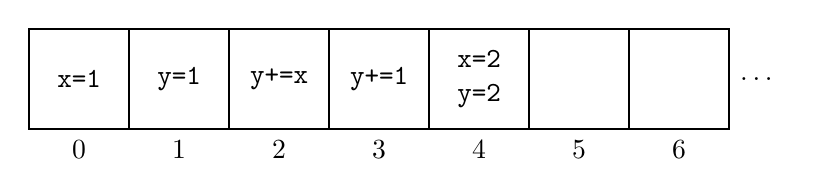
\begin{tikzpicture}
    \node[square] (a) at (0, 0) {\texttt{x=1}};
    \node[square, right=-1pt of a] (b) {\texttt{y=1}};
    \node[square, right=-1pt of b] (c) {\texttt{y+=x}};
    \node[square, right=-1pt of c] (d) {\texttt{y+=1}};
    \node[square, right=-1pt of d] (e) {\texttt{x=2\\y=2}};
    \node[square, right=-1pt of e] (f) {};
    \node[square, right=-1pt of f] (g) {};
    \node[right=0in of g] (h) {\ldots};

    \foreach \label/\i in {a/0, b/1, c/2, d/3, e/4, f/5, g/6} {%
      \node[below=0in of \label] {\i};
    }
  \end{tikzpicture}
  \caption{MultiPaxos}\figlabel{MultiPaxosCartoon}
\end{figure}

While simple, agreeing on a totally ordered sequence of state machine commands
can be overly prescriptive. If two commands conflict (e.g., \texttt{x = 1} and
\texttt{x = 2}), then they \emph{do} need to be executed by every state machine
replica in the same order. But, if two commands do \emph{not} conflict (e.g.,
\texttt{x = 1} and \texttt{y = 1}), then they do \emph{not} need to be totally
ordered.  State machine replicas can execute them in either order.

EPaxos takes advantage of this fact and attempts to order commands only if they
conflict. To do so, it ditches the totally ordered sequence and instead agrees
on a directed graph of commands such that every pair of conflicting commands
have an edge between them. An example is illustrated in \figref{EPaxosCartoon}%
\footnote{%
  In reality, the graph would be the transitive closure of the one in
  \figref{EPaxosCartoon}, but we do not draw all edges to keep things simple
}.
EPaxos then executes this graph in reverse topological order one strongly
connected component at a time, executing commands within a component in an
arbitrary but deterministic order. For example, in \figref{EPaxosCartoon}, we
could execute commands in the order $R.1, R.2, S.1, Q.2, Q.1$.

\begin{figure}[h]
  \centering
  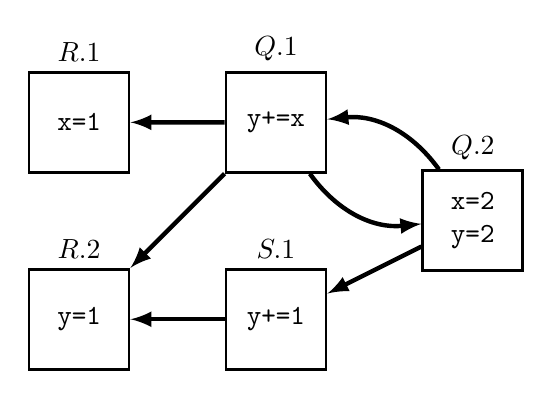
\begin{tikzpicture}[scale=2.5]
    \node[square] (a) at (0, 1) {\texttt{x=1}};
    \node[square] (b) at (0, 0) {\texttt{y=1}};
    \node[square] (c) at (1, 1) {\texttt{y+=x}};
    \node[square] (d) at (1, 0) {\texttt{y+=1}};
    \node[square] (e) at (2, 0.5) {\texttt{x=2\\y=2}};
    \draw[ultra thick, -latex] (c) to (a);
    \draw[ultra thick, -latex] (c) to (b);
    \draw[ultra thick, -latex, bend right] (c) to (e);
    \draw[ultra thick, -latex] (d) to (b);
    \draw[ultra thick, -latex, bend right] (e) to (c);
    \draw[ultra thick, -latex] (e) to (d);

    \foreach \label/\i in {a/$R.1$, b/$R.2$, c/$Q.1$, d/$S.1$, e/$Q.2$} {%
      \node[above=0in of \label] {\i};
    }
  \end{tikzpicture}
  \caption{EPaxos}\figlabel{EPaxosCartoon}
\end{figure}

Every vertex in the graph has a unique name like $Q.1$ or $R.1$. EPaxos calls
these \defword{instances}. We can view a named vertex, the command inside the
vertex, and the vertex's outbound edges as a little gadget. For example,
\figref{EPaxosGadgets} shows gadgets for instances $R.2$, $Q.1$, and $Q.2$.
%
More formally, we can think of these gadgets as tuples like $(Q.1,
\texttt{y+=x}, \set{R.1, R.2, Q.2})$ where $Q.1$ is the instance, \texttt{y+=x}
is the command in the instance, and the set $\set{R.1, R.2, Q.2}$ is the set of
\defword{dependencies} of $Q.1$ (or of \texttt{y+=x} if $Q.1$ is clear from
context).

\begin{figure}[h]
  \centering

  \begin{subfigure}[b]{0.19\textwidth}
    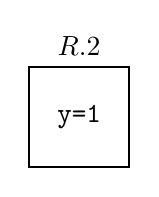
\begin{tikzpicture}[scale=2.5]
      \node[square] (b) at (0, 0) {\texttt{y=1}};
      \foreach \label/\i in {b/$R.2$} {%
        \node[above=0in of \label] {\i};
      }
    \end{tikzpicture}
  \end{subfigure}
  %
  \begin{subfigure}[b]{0.49\textwidth}
    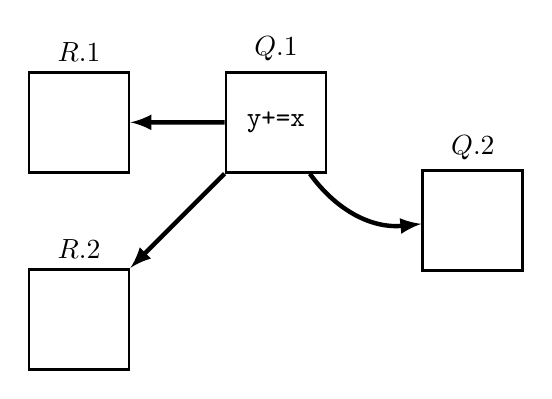
\begin{tikzpicture}[scale=2.5]
      \node[square] (a) at (0, 1) {};
      \node[square] (b) at (0, 0) {};
      \node[square] (c) at (1, 1) {\texttt{y+=x}};
      \node[square] (e) at (2, 0.5) {};
      \draw[ultra thick, -latex] (c) to (a);
      \draw[ultra thick, -latex] (c) to (b);
      \draw[ultra thick, -latex, bend right] (c) to (e);
      \foreach \label/\i in {a/$R.1$, b/$R.2$, c/$Q.1$, e/$Q.2$} {%
        \node[above=0in of \label] {\i};
      }
    \end{tikzpicture}
  \end{subfigure}
  %
  \begin{subfigure}[b]{0.29\textwidth}
    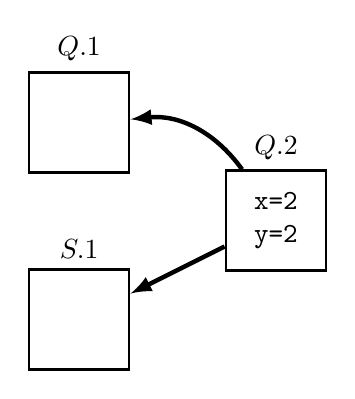
\begin{tikzpicture}[scale=2.5]
      \node[square] (c) at (1, 1) {};
      \node[square] (d) at (1, 0) {};
      \node[square] (e) at (2, 0.5) {\texttt{x=2\\y=2}};
      \draw[ultra thick, -latex, bend right] (e) to (c);
      \draw[ultra thick, -latex] (e) to (d);
      \foreach \label/\i in {c/$Q.1$, d/$S.1$, e/$Q.2$} {%
        \node[above=0in of \label] {\i};
      }
    \end{tikzpicture}
  \end{subfigure}

  \caption{EPaxos Gadgets}\figlabel{EPaxosGadgets}
\end{figure}

EPaxos nodes collectively construct the directed graph of commands by stitching
together a bunch of gadgets. More precisely, an EPaxos node $R$ proposes a
gadget for instance $R.i$ and attempts to get the gadget chosen. Once a gadget
is chosen, it is considered part of the directed graph and is eligible for
execution. EPaxos' correctness hinges on the following two key invariants
(later we'll see why these invariants ensure EPaxos' correctness).

\begin{boxedinvariant}\invlabel{GadgetsChosen}
  Once a gadget $(R.i, a, \deps{a})$ has been chosen, no other gadget can be
  chosen for instance $R.i$.
\end{boxedinvariant}

\begin{boxedinvariant}\invlabel{ConflictingGadgets}
  If two gadgets $(I_a, a, \deps{a})$ and $(I_b, b, \deps{b})$ are chosen and
  commands $a$ and $b$ conflict, then either $I_a \in \deps{b}$ or $I_b \in
  \deps{a}$ or both.
\end{boxedinvariant}

BPaxos, like EPaxos, also constructs a directed graph of commands and executes
them in reverse topological order one strongly connected component at a time.
In fact, BPaxos and EPaxos execute commands in 100\% the same way. BPaxos also
maintains the same two key invariants as EPaxos. BPaxos and EPaxos differ only
in how they construct the directed graph of commands.
%
BPaxos is illustrated in \figref{BPaxos}. A BPaxos instance has three main
components: an ordering service, a consensus service, and a set of BPaxos
nodes. The ordering service helps provide \invref{ConflictingGadgets}, the
consensus service helps provide \invref{GadgetsChosen}, and the BPaxos nodes
glue the two together. We explain each of these three components in turn.

{\section{Bipartisan Paxos}
BPaxos is a modular state machine replication protocol that is both multileader
and generalized. Throughout the paper, we make the standard assumptions that
the network is asynchronous, that state machines are deterministic, and that
machines can fail by crashing but cannot act maliciously. We also assume that
at most $f$ machines can fail for some integer-valued parameter $f$. Throughput
the paper, we omit low-level protocol details involving the re-sending of
dropped messages.

\subsection{Goodbye Logs, Hello Graphs}
MultiPaxos is \emph{not} generalized. It totally orders all commands by
sequencing them into a \emph{log}. BPaxos is generalized, so it ditches the log
and instead partially orders commands into a \emph{directed graph}, like the
ones shown in \figref{ExampleBPaxosExecution}.

BPaxos graphs are completely analogous to MultiPaxos logs. Every MultiPaxos log
entry corresponds to a \defword{vertex} in a BPaxos graph. Every MultiPaxos log
entry holds a command; so does every vertex. Every log entry is uniquely
identified by it's index (e.g., \textcolor{flatred}{$0$}); every vertex is
uniquely identified by a \defword{vertex id} (e.g.,
\textcolor{flatred}{$v_0$}). The one difference between graphs and logs are the
edges. Every BPaxos vertex $v$ has edges to some set of other vertices. These
edges are called the \defword{dependencies} of $v$. Note that we view a
vertex's dependencies as belonging to the vertex, so when we refer to a vertex,
we are also referring to its dependencies. The similarities between MultiPaxos
logs and BPaxos graphs are summarized in \tabref{MultiPaxosVsBPaxos}.

\begin{table}[ht]
  \centering
  \caption{A comparison of MultiPaxos log entries and BPaxos vertices.}
  \tablabel{MultiPaxosVsBPaxos}
  \begin{tabular}{r|l}
    \textbf{BPaxos} & \textbf{MultiPaxos} \\\hline
    graph           & log \\
    vertex          & log entry \\
    vertex id       & index \\
    command         & command \\
    dependencies    & - \\
  \end{tabular}
\end{table}

MultiPaxos grows its \emph{log} over time by repeatedly reaching consensus on
one \emph{log entry} at a time. BPaxos grows its \emph{graph} over time by
repeatedly reaching consensus on one \emph{vertex} (and its dependencies) at a
time. MultiPaxos replicas execute logs in prefix order, making sure not to
execute a command until after executing \emph{all previous commands}. BPaxos
replicas execute graphs in prefix order (i.e. reverse topological order),
making sure not to execute a command until after executing \emph{its
dependencies}.

An example of how BPaxos graphs grow over time and how a BPaxos replica
executes these graphs in shown in \figref{ExampleBPaxosExecution}. As you read
through the figure, note the similarities with
\figref{ExampleMultiPaxosExecution}.
%
First, the command $a \gets 0$ is chosen in vertex $v_0$ with no dependencies
(\figref{ExampleBPaxosExecutionA}).
%
Because the vertex has no dependencies, the replica executes $a \gets 0$
immediately (\figref{ExampleBPaxosExecutionB}).
%
Next, the command $a \gets b$ is chosen in vertex $v_2$ with dependencies on
vertices $v_0$ and $v_1$ (\figref{ExampleBPaxosExecutionC}).
%
$v_2$ depends on $v_1$, but a command has not yet been chosen in $v_1$, so the
replica does \emph{not} yet execute $a \gets b$
(\figref{ExampleBPaxosExecutionD}).
%
Finally, the command $b \gets 0$ is chosen in vertex $v_1$ with no
dependencies (\figref{ExampleBPaxosExecutionE}).
%
Because $b \gets 0$ has no dependencies, the replica executes it immediately.
Moreover, all of $v_2$'s dependencies have been executed, so the replica now
executes $a \gets b$ (\figref{ExampleBPaxosExecutionF}).

{\newlength{\vertexinnersep}
\setlength{\vertexinnersep}{2pt}
\newlength{\vertexlinewidth}
\setlength{\vertexlinewidth}{1pt}
\newlength{\vertexwidth}
\setlength{\vertexwidth}{\widthof{$a \gets 1$}+2\vertexinnersep}
\newcommand{\graphindexcolor}{flatred}
\newcommand{\cmdi}{$a \gets 0$}
\newcommand{\cmdii}{$b \gets 0$}
\newcommand{\cmdiii}{$a \gets b$}
\newcommand{\xscale}{0.8}
\newcommand{\yscale}{0.75}

\tikzstyle{vertex}=[draw,
                      inner sep=\vertexinnersep,
                      line width=\vertexlinewidth,
                      minimum height=\vertexwidth,
                      minimum width=\vertexwidth]

\tikzstyle{executed}=[fill=gray, opacity=0.2, draw opacity=1, text opacity=1]

\tikzstyle{dep}=[-latex, thick]

\tikzstyle{graphindex}=[\graphindexcolor]

\begin{figure}
  \begin{subfigure}[t]{0.45\columnwidth}
    \centering
    \begin{tikzpicture}[xscale=\xscale, yscale=\yscale]
      \node[vertex, label={[graphindex]90:$v_0$}] (0) at (0, 2) {\cmdi{}};
    \end{tikzpicture}
    \caption{%
      \cmdi{} is chosen in entry $\textcolor{\graphindexcolor}{v_0}$.
    }
    \figlabel{ExampleBPaxosExecutionA}
  \end{subfigure}\hspace{0.1\columnwidth}%
  \begin{subfigure}[t]{0.45\columnwidth}
    \centering
    \begin{tikzpicture}[xscale=\xscale, yscale=\yscale]
      \node[vertex, executed, label={[graphindex]90:$v_0$}] (0) at (0, 2)
        {\cmdi{}};
    \end{tikzpicture}
    \caption{%
      \cmdi{} is executed.
    }
    \figlabel{ExampleBPaxosExecutionB}
  \end{subfigure}

  \vspace{2pt}\textcolor{flatgray}{\rule{\columnwidth}{0.4pt}}

  \begin{subfigure}[t]{0.45\columnwidth}
    \centering
    \begin{tikzpicture}[xscale=\xscale, yscale=\yscale]
      \node[vertex, executed, label={[graphindex]90:$v_0$}] (0) at (0, 2)
        {\cmdi{}};
      \node[vertex, label={[graphindex]90:$v_2$}] (2) at (2, 1) {\cmdiii{}};
      \node[vertex, label={[graphindex]90:$v_1$}] (1) at (0, 0) {};
      \draw[dep] (2) to (0);
      \draw[dep] (2) to (1);
    \end{tikzpicture}
    \caption{%
      \cmdiii{} is chosen in entry $\textcolor{\graphindexcolor}{v_2}$.
    }
    \figlabel{ExampleBPaxosExecutionC}
  \end{subfigure}\hspace{0.1\columnwidth}%
  \begin{subfigure}[t]{0.45\columnwidth}
    \centering
    \begin{tikzpicture}[xscale=\xscale, yscale=\yscale]
      \node[vertex, executed, label={[graphindex]90:$v_0$}] (0) at (0, 2)
        {\cmdi{}};
      \node[vertex, label={[graphindex]90:$v_2$}] (2) at (2, 1) {\cmdiii{}};
      \node[vertex, label={[graphindex]90:$v_1$}] (1) at (0, 0) {};
      \draw[dep] (2) to (0);
      \draw[dep] (2) to (1);
    \end{tikzpicture}
    \caption{%
      Nothing is executed.
    }
    \figlabel{ExampleBPaxosExecutionD}
  \end{subfigure}

  \vspace{2pt}\textcolor{flatgray}{\rule{\columnwidth}{0.4pt}}

  \begin{subfigure}[t]{0.45\columnwidth}
    \centering
    \begin{tikzpicture}[xscale=\xscale, yscale=\yscale]
      \node[vertex, executed, label={[graphindex]90:$v_0$}] (0) at (0, 2)
        {\cmdi{}};
      \node[vertex, label={[graphindex]90:$v_2$}] (2) at (2, 1) {\cmdiii{}};
      \node[vertex, label={[graphindex]90:$v_1$}] (1) at (0, 0) {\cmdii{}};
      \draw[dep] (2) to (0);
      \draw[dep] (2) to (1);
    \end{tikzpicture}
    \caption{%
      \cmdii{} is chosen in entry $\textcolor{\graphindexcolor}{v_1}$.
    }
    \figlabel{ExampleBPaxosExecutionE}
  \end{subfigure}\hspace{0.1\columnwidth}%
  \begin{subfigure}[t]{0.45\columnwidth}
    \centering
    \begin{tikzpicture}[xscale=\xscale, yscale=\yscale]
      \node[vertex, executed, label={[graphindex]90:$v_0$}] (0) at (0, 2)
        {\cmdi{}};
      \node[vertex, executed, label={[graphindex]90:$v_2$}] (2) at (2, 1)
        {\cmdiii{}};
      \node[vertex, executed, label={[graphindex]90:$v_1$}] (1) at (0, 0)
        {\cmdii{}};
      \draw[dep] (2) to (0);
      \draw[dep] (2) to (1);
    \end{tikzpicture}
    \caption{%
      \cmdii{}, \cmdiii{} are executed.
    }
    \figlabel{ExampleBPaxosExecutionF}
  \end{subfigure}

  \caption{%
    An example of a BPaxos replica executing commands over time, as they are
    chosen.
  }
  \figlabel{ExampleBPaxosExecution}
\end{figure}
}

Before we discuss the mechanisms that BPaxos uses to construct these graphs,
note the following three graph properties.

\paragraph{Vertices are chosen once and for all}
BPaxos reaches consensus on every vertex, so once a vertex has been chosen, it
will never change. It's command won't change, it won't lose dependencies,
and it won't get new dependencies.

\paragraph{Cycles can happen, but aren't a problem}
We'll see in a moment that BPaxos graphs can sometimes be cyclic. These cycles
are a nuisance, but easily handled. Instead of executing graphs in reverse
topological order one \emph{command} at a time, replicas instead execute graphs
in reverse topological order one \emph{strongly connected component} at a time.
The commands within a strongly connected component are executed in an arbitrary
yet deterministic order (e.g., in vertex id order). This is illustrated in
\figref{ExampleBPaxosCycleExecution}.

{\newlength{\cyclevertexinnersep}
\setlength{\cyclevertexinnersep}{4pt}
\newlength{\cyclevertexlinewidth}
\setlength{\cyclevertexlinewidth}{1pt}
\newlength{\cyclevertexwidth}
\setlength{\cyclevertexwidth}{\widthof{$x$}+2\cyclevertexinnersep}
\newcommand{\graphindexcolor}{flatred}
\newcommand{\cmdi}{$a \gets 0$}
\newcommand{\cmdii}{$b \gets 0$}
\newcommand{\cmdiii}{$a \gets b$}
\newcommand{\xscale}{0.5}
\newcommand{\yscale}{0.5}

\tikzstyle{vertex}=[draw,
                    inner sep=\cyclevertexinnersep,
                    line width=\cyclevertexlinewidth,
                    minimum height=\cyclevertexwidth,
                    minimum width=\cyclevertexwidth]

\tikzstyle{executed}=[fill=gray, opacity=0.2, draw opacity=1, text opacity=1]

\tikzstyle{dep}=[-latex, thick]

\tikzstyle{graphindex}=[\graphindexcolor]

\begin{figure}
  \centering

  \begin{subfigure}[t]{0.3\columnwidth}
    \centering
    \begin{tikzpicture}[xscale=\xscale, yscale=\yscale]
      \node[vertex, executed, label={[graphindex]90:$v_x$}] (x) at (0, 1) {$x$};
      \node[vertex, label={[graphindex]90:$v_y$}] (y) at (2, 2) {$y$};
      \node[vertex, label={[graphindex]-90:$v_z$}] (z) at (2, 0) {};
      \draw[dep] (y) to (x);
      \draw[dep, bend left] (y) to (z);
    \end{tikzpicture}
    \caption{}
    \figlabel{ExampleBPaxosCycleExecutionA}
  \end{subfigure}\hspace{0.04\columnwidth}%
  \begin{subfigure}[t]{0.3\columnwidth}
    \centering
    \begin{tikzpicture}[xscale=\xscale, yscale=\yscale]
      \node[vertex, executed, label={[graphindex]90:$v_x$}] (x) at (0, 1) {$x$};
      \node[vertex, label={[graphindex]90:$v_y$}] (y) at (2, 2) {$y$};
      \node[vertex, label={[graphindex]-90:$v_z$}] (z) at (2, 0) {$z$};
      \draw[dep] (y) to (x);
      \draw[dep, bend left] (y) to (z);
      \draw[dep, bend left] (z) to (y);
    \end{tikzpicture}
    \caption{}
    \figlabel{ExampleBPaxosCycleExecutionB}
  \end{subfigure}\hspace{0.04\columnwidth}%
  \begin{subfigure}[t]{0.3\columnwidth}
    \centering
    \begin{tikzpicture}[xscale=\xscale, yscale=\yscale]
      \node[vertex, executed, label={[graphindex]90:$v_x$}] (x) at (0, 1) {$x$};
      \node[vertex, executed, label={[graphindex]90:$v_y$}] (y) at (2, 2) {$y$};
      \node[vertex, executed, label={[graphindex]-90:$v_z$}] (z) at (2, 0) {$z$};
      \draw[dep] (y) to (x);
      \draw[dep, bend left] (y) to (z);
      \draw[dep, bend left] (z) to (y);
    \end{tikzpicture}
    \caption{}
    \figlabel{ExampleBPaxosCycleExecutionB}
  \end{subfigure}

  \caption{%c
    An example of a BPaxos replica executing a cyclic graph.
    (a) $y$ cannot be exeucted until $v_z$ is chosen.
    (b) $v_z$ is chosen. $v_y$ and $v_z$ form a strongly connected component.
    (c) $y$ and $z$ are executed in an arbitrary yet deterministic order; $y$
        then $z$ or $z$ then $y$.%
  }
  \figlabel{ExampleBPaxosCycleExecution}
\end{figure}
}

\paragraph{Conflicting commands depend on each other}
Because BPaxos is generalized, only conflicting commands have to be ordered
with respect to each other. BPaxos ensures this by maintaining the following
invariant:
\begin{invariant}[\defword{dependency invariant}]\invlabel{KeyInvariant}
  If two conflicting commands $x$ and $y$ are chosen in vertices $v_x$ and
  $v_y$, then either $v_x$ depends on $v_y$ or $v_y$ depends on $v_x$ or both.
  That is, there is at least one edge between vertices $v_x$ and $v_y$.
\end{invariant}
Because every conflicting pair of commands has an edge between them, every
replica is guaranteed to execute the commands in the same order.
Non-conflicting commands do not need an edge between them and can be executed
in either order.

\subsection{Protocol Overview}
BPaxos is composed of five modules: a dependency service, a consensus service,
a set of leaders, a set of proposers, and a set of replicas. Here, we give an
overview on how these modules interact by walking through the example execution
shown in \figref{BPaxosOverview}. In the next couple of sections, we discuss
each module in more detail.

1. A client $c$ sends a state machine command $x$ to leader $l_0$. Note that
all of the leaders process commands in parallel and that clients can send
commands to any of them.

2. Upon receiving command $x$, $l_0$ generates a globally unique vertex id
$v_x$ for $x$. It then sends the message $\msg{v_x, x}$ to the dependency
service.

3. Upon receiving message $\msg{v_x, x}$, the dependency service computes a set
of dependencies $\deps{}_x$ for vertex $v_x$. It sends back the message
$\msg{v_x, x, \deps{}_x}$ to $l_0$.

4. $l_0$ forwards $\msg{v_x, x, \deps{}_x}$ to proposer $p_0$.

5. $p_0$ sends the message $\msg{v_x, x, \deps{}_x}$ to the consensus service,
proposing that the value $(x, \deps{}_x)$ be chosen in vertex $v_x$.

6. The consensus service implements one instance of consensus for every vertex.
Upon receiving $\msg{v_x, x, \deps{}_x}$, it chooses the value $(x, \deps{}_x)$
for vertex $v_x$ and notifies $p_0$ with the message $\msg{v_x, x, \deps{}_x}$.
Note that in this example, the consensus service chose the value proposed by
$p_0$. In general, the consensus service may choose some other value if other
proposers are concurrently proposing different values for vertex $v_x$.
However, we'll see later that this can only happen during recovery, and is
therefore not typical.

7. After $p_0$ learns that command $x$ with dependencies $\deps{}_x$ has been
chosen in vertex $v_x$, it notifies the replicas by sending the message
$\msg{v_x, x, \deps{}_x}$.

8. Every replica manages a graph of chosen commands. Upon receiving $\msg{v_x,
x, \deps{}_x}$, the replicas add the vertex $v_x$ to their graph with command
$x$ and dependencies $\deps{}_x$. As described earlier, the replicas execute
the graph in reverse topological order. Once they've executed command $x$,
yielding output $o$, one of the replicas sends back the response to the client
$c$.

{\input{figures/common.tex}

\tikzstyle{proc}=[draw, circle, thick, inner sep=2pt]
\tikzstyle{leader}=[proc, fill=\leadercolor!25]
\tikzstyle{proposer}=[proc, fill=\proposercolor!25]
\tikzstyle{replica}=[proc, fill=\replicacolor!25]
\tikzstyle{client}=[proc, fill=\clientcolor!25]
\tikzstyle{proclabel}=[inner sep=0pt]
\tikzstyle{fakeproclabel}=[inner sep=0pt, white]
\tikzstyle{comm}=[-latex, thick]
\tikzstyle{commnum}=[fill=white, inner sep=0pt]
\tikzstyle{service}=[draw, rounded corners, align=center, thick]
\tikzstyle{depservice}=[service, draw=\depservicecolor!50]
\tikzstyle{consensus}=[service, draw=\consensuscolor]
\tikzstyle{module}=[draw, thick, flatgray, rounded corners]

\begin{figure}[t]
  \centering

  \begin{tikzpicture}[yscale=0.9, xscale=0.70]
    % Nodes
    \node[client] (c) at (0, 1.5) {$c$};
    \node[leader] (l0) at (2, 3) {$l_0$};
    \node[leader] (l1) at (4, 3) {$l_1$};
    \node[proposer] (p0) at (2, 1.5) {$p_0$};
    \node[proposer] (p1) at (4, 1.5) {$p_1$};
    \node[replica] (r0) at (2, 0) {$r_0$};
    \node[replica] (r1) at (4, 0) {$r_1$};
    \node[depservice] (depservice) at (0, 5) {Dependency\\Service};
    \node[consensus] (consensus) at (4, 5) {Consensus\\Service};

    % Modules
    \draw[module, \leadercolor!25]
      ($(l0.south west) + (-0.25, -0.25)$) rectangle
      ($(l1.north east) + (0.25, 0.25)$);
      \draw[module, \proposercolor!25]
      ($(p0.south west) + (-0.25, -0.25)$) rectangle
      ($(p1.north east) + (0.25, 0.25)$);
    \draw[module, \replicacolor!25]
      ($(r0.south west) + (-0.25, -0.25)$) rectangle
      ($(r1.north east) + (0.25, 0.25)$);

    % Labels
    \draw[black!100, comm] (c) to node[commnum]{$1$} (l0);
    \draw[black!85, comm, bend left=10] (l0) to node[commnum]{$2$} (depservice);
    \draw[black!85, comm, bend left=10] (depservice) to node[commnum]{$3$} (l0);
    \draw[black!85, comm] (l0) to node[commnum]{$4$} (p0);
    \draw[black!85, comm] (p0) to node[commnum]{$5$} (consensus);
    \draw[black!80, comm, bend left=15] (consensus) to node[commnum]{$6$} (p0);
    \draw[black!80, comm] (p0) to node[commnum]{$7$} (r0);
    \draw[black!80, comm] (p0) to node[commnum]{$7$} (r1);
    \draw[black!80, comm] (r0) to node[commnum]{$8$} (c);

    % Labels
    \node[fakeproclabel, anchor=west] (leaders) at (5, 3) {$\geq f+1$ Leaders};
    \halffill{leaders}{\leadercolor!25}
    \node[proclabel, anchor=west] at (leaders.west) {$\geq f+1$ Leaders};

    \node[fakeproclabel, anchor=west] (proposers) at (5, 1.5) {$\geq f+1$ Proposers};
    \halffill{proposers}{\proposercolor!25}
    \node[proclabel, anchor=west] at (proposers.west) {$\geq f+1$ Proposers};

    \node[fakeproclabel, anchor=west] (replicas) at (5, 0) {$\geq f+1$ Replicas};
    \halffill{replicas}{\replicacolor!25}
    \node[proclabel, anchor=west] at (replicas.west) {$\geq f+1$ Replicas};

    % Legend.
    \node[align=left, anchor=east] at ($(c.west)+(-0.5, 0.5)$) {%
      \textbf{Legend} \\
      $1$: $x$ \\
      $2$: $\msg{v_x, x}$ \\
      $3$: $\msg{v_x, x, \deps{}_x}$ \\
      $4$: $\msg{v_x, x, \deps{}_x}$ \\
      $5$: $\msg{v_x, x, \deps{}_x}$ \\
      $6$: $\msg{v_x, x, \deps{}_x}$ \\
      $7$: $\msg{v_x, x, \deps{}_x}$ \\
      $8$: $o$
    };
  \end{tikzpicture}

  \caption{An overview of BPaxos execution}
  \figlabel{BPaxosOverview}
\end{figure}
}

\subsection{Dependency Service}
When the dependency service receives a message of the form $\msg{v_x, x}$, it
replies with a set of dependencies $\deps{}_x$ for $v_x$ using the message
$\msg{v_x, x, \deps{}_x}$. The dependency service maintains the following
invariant.

\begin{invariant}[\defword{dependency service invariant}]%
  \invlabel{DepServiceInvariant}
  If the dependency service produces responses $\msg{v_x, x, \deps{}_x}$ and
  $\msg{v_y, y, \deps{}_y}$ for conflicting commands $x$ and $y$, then $v_x \in
  \deps{}_y$ or $v_y \in \deps{}_x$ or both.
\end{invariant}

That is, the dependency service computes dependencies such that conflicting
commands depend on each other. Note that the dependency service invariant
(\invref{DepServiceInvariant}) is very similar to the dependency invariant
(\invref{KeyInvariant}). This is not an accident. Only dependencies computed by
the dependency service can be chosen, so the dependency service invariant
suffices to guarantee that the dependency invariant is maintained.

Concretely, we implement the dependency service with $2f+1$ dependency service
nodes. Every dependency service node maintains a single piece of state,
\textsf{commands}. \textsf{commands} is the set of all the messages that the
dependency service node has received to date. When a dependency service node
receives message $\msg{v_x, x}$ from a leader, it computes
\[
  \deps{} = \setst{y}{\msg{v_y, y} \in \textsf{commands}
                      ~\text{and $x$ and $y$ conflict}}.
\]
It then adds $\msg{v_x, x}$ to \textsf{commands} and sends $\msg{v_x, x,
\deps{}}$ to the leader. When a leader sends a message $\msg{v_x, x}$ to the
dependency service, it sends it to every dependency service node. Upon
receiving $f + 1$ responses, $\set{\msg{v_x, x, \deps{}_1}, \ldots, \msg{v_x, x,
\deps{}_{f+1}}}$, the leader computes the final dependencies as
$\bigcup_{i=1}^{f+1} \deps{}_i$, the union of the computed dependencies.

\begin{theorem}
  The dependency service maintains \invref{DepServiceInvariant}.
\end{theorem}
\begin{proof}
  Assume the dependency service produces responses $\msg{v_x, x, \deps{}_x}$ and
  $\msg{v_y, y, \deps{}_y}$ for conflicting commands $x$ and $y$. We want to
  show that $v_x \in \deps{}_y$ or $v_y \in \deps{}_x$ or both. $\deps{}_x$ is
  the union of dependencies computed by some set $Q_x$ of $f + 1$ dependency
  service nodes. Similarly, $\deps{}_y$ is the union of dependencies computed
  by some set $Q_y$ of $f + 1$ dependency service nodes. Any two sets of $f +
  1$ nodes must intersect ($f+1$ is a majority of $2f+1$). Consider a
  dependency service node $d$ in the intersection of $Q_x$ and $Q_y$. $d$
  received both $\msg{v_x, x}$ and $\msg{v_y, y}$. Without loss of generality,
  assume it received $\msg{v_y, y}$ second. Then, when $d$ received $\msg{v_y,
  y}$, $\msg{v_x, x}$ was already in its \textsf{commands}, so it must have
  included $v_x$ in its computed dependencies for $v_y$. $\deps{}_y$ is a union
  of dependencies that includes the dependencies computed by $d$. Thus, $v_x
  \in \deps{}_y$.
\end{proof}

Note that if the dependency service produces responses $\msg{v_x, x,
\deps{}_x}$ and $\msg{v_y, y, \deps{}_y}$ for conflicting commands $x$ and $y$,
it may include $v_x \in \deps{}_y$ \emph{and} $v_y \in \deps{}_x$. For example,
if dependency service node $d_1$ receives $x$ then $y$ while dependency service
node $d_2$ receives $y$ then $x$, then dependencies formed from $d_1$ and $d_2$
will have $v_x$ and $v_y$ in each other's dependencies. This is the reason why
BPaxos graphs may develop cycles.

\subsection{Leaders}
The dependency

\subsection{Proposers and Consensus Service}
mention you can use paxos with proposers being paxos proposers and this service
implemented as paxos acceptors


\subsection{Recovery}

add pseudocode (including dep service) jk
add protocol diagram

{% https://tex.stackexchange.com/a/226010
\newcommand{\LineComment}[1]{\textcolor{gray}{// #1}}

\tikzstyle{comm}=[-latex, thick]
\tikzstyle{commnum}=[fill=white, inner sep=1pt]
\tikzstyle{proc}=[thick, text width=0.45\textwidth, anchor=north]

\begin{figure*}[t]
  \centering
  \begin{tikzpicture}
    \node[draw,
          thick,
          minimum width=6.8in,
          minimum height=0.25in]
          (clients) at (4.5, 1.25) {\large \textbf{Clients}};

    \node[proc,
          draw=\leadercolor,
          label={90:\textbf{\large Leader}}] (leader) at (0, 0) {%
      \newcommand{\leaderindex}{\textsf{leader index}}
      \newcommand{\nextid}{\textsf{next id}}
      \begin{algorithmic}[1]
        \GlobalState $\leaderindex{}$ \LineComment{e.g., $l_0$ has index $0$}
        \GlobalState $\nextid{} \gets 0$
        \Upon{receiving command $x$ from client}
          \State $v_x \gets (\leaderindex{}, \nextid{})$
          \State $\nextid{} \gets \nextid + 1$
          \State send $\msg{v_x, x}$ to dependency service nodes
        \EndUpon
        \Upon{receiving dependencies from $f + 1$ dependency service nodes for vertex $v_x$}
          \State let $\deps{}_1, \ldots, \deps{}_{f+1}$ be the dependencies
          \State $\deps{}_x \gets \bigcup_i \deps{}_i$
          \State send $\msg{v_x, x, \deps{}_x}$ to a proposer
        \EndUpon
      \end{algorithmic}
    };

    \node[proc,
          draw=\depservicecolor,
          label={90:\textbf{\large Dependency Service Node}},
          anchor=north] (depservice) at (9, 0) {%
      \newcommand{\commands}{\textsf{cmds}}
      \begin{algorithmic}[1]
        \GlobalState $\commands$ \LineComment{set of messages $\msg{v_x, x}$}
        \Upon{receiving $\msg{v_x, x}$ from leader $l$}
          \State $\deps{} = \setst{v_y}{\msg{v_y, y} \in \commands \land
                                        \text{$x$, $y$ conflict}}$
          \State send $\msg{v_x, x, \deps{}}$ to $l$
        \EndUpon
      \end{algorithmic}
    };

    \node[proc,
          draw=\proposercolor,
          label={90:\textbf{\large Proposer}},
          below=of leader] (proposer) {%
      \begin{algorithmic}[1]
        \Upon{receiving $\msg{v_x, x, \deps{}_x}$ from leader}
          \State send $\msg{v_x, x, \deps{}_x}$ to consensus service
        \EndUpon

        \Upon{receiving $\msg{v_x, x, \deps{}_x}$ from consensus service}
          \State send $\msg{v_x, x, \deps{}_x}$ to replicas
        \EndUpon
      \end{algorithmic}
    };

    \node[proc,
          draw=\consensuscolor,
          label={90:\textbf{\large Consensus Service}},
          below=of depservice] (consensus) {%
      \begin{algorithmic}[1]
        \Upon{receiving $\msg{v_x, x, \deps{}_x}$ from proposer $p$}
          \State reach consensus on $(x', \deps{}_x')$ for vertex $v_x$
          \State send $\msg{v_x, x', \deps{}_x'}$ to $p$
        \EndUpon
      \end{algorithmic}
    };

    \node[proc,
          draw=\replicacolor,
          label={90:\textbf{\large Replica}},
          below=of consensus] (replica) {%
      \newcommand{\graph}{\textsf{graph}}
      \newcommand{\replicaIndex}{\textsf{replica index}}
      \newcommand{\numReplicas}{\textsf{num replicas}}
      \begin{algorithmic}[1]
        \GlobalState $\graph$ \LineComment{BPaxos graph of chosen vertices}
        \GlobalState $\numReplicas{}$ \LineComment{the number of replicas}
        \Upon{receiving $\msg{v_x, x, \deps{}_x}$ from proposer}
          \State add $\msg{v_x, x, \deps{}_x}$ to $\graph$
          \State execute every eligible vertex $v_y$
          \If{$\text{hash}(v_y)~\%~\numReplicas = \replicaIndex$}
            \State send result of executing $v_y$ back to client
          \EndIf
        \EndUpon
      \end{algorithmic}
    };

    \draw[comm]
      ($(clients.south west)!0.72!(clients.south)$)
      to node[commnum] {$1$}
      ($(leader.north)!0.5!(leader.north east)$);
    \draw[comm, black!85]
      ($(leader.north east)!0.5!(leader.east)$)
      to node[commnum] {$2$}
      (depservice);
    \draw[comm, black!85]
      (depservice.south west) to node[commnum] {$3$} (leader.east);
    \draw[comm, black!85]
      ($(leader.south)!0.5!(leader.south east)$)
      to node[commnum] {$4$}
      ($(proposer.north)!0.5!(proposer.north east)$);
    \draw[comm, black!80] (proposer.north east) to node[commnum] {$5$} (consensus.west);
    \draw[comm, black!80] (consensus) to node[commnum] {$6$} (proposer.north east);
    \draw[comm, black!80] (proposer) to node[commnum] {$7$} (replica);
    \draw[comm, black!80]
      (replica.east) to ++(0.5, 0)
                     to node[commnum]{$8$} ++(0, 8.75)
                     to (clients.east);
  \end{tikzpicture}

  \caption{BPaxos pseudocode}
  \figlabel{BPaxosPseudocode}
\end{figure*}
}
}

\paragraph{Ordering Service}
The ordering service is responsible for computing the dependencies between
conflicting state machine commands. When a BPaxos node $R$ receives a state
machine command $a$ from a client, it chooses some instance $R.i$ for $a$.
Then, $R$ sends $a$ and $R.i$ to the ordering service. When the ordering
service receives a command $a$ for instance $R.i$, it replies with a tuple
$(R.i, a, \deps{a})$ where $\deps{a} = \set{I_1, \ldots, I_n}$ is $a$'s
dependencies.
%
The ordering service maintains the following invariant.

\begin{boxedinvariant}\invlabel{OrderingService}
If two conflicting commands $a$ and $b$ in instances $I_a$ and $I_b$ yield
responses $(I_a, a, \deps{a})$ and $(I_b, b, \deps{b})$ from the ordering
service, then either $I_a \in \deps{b}$ or $I_b \in \deps{a}$ (or both). That
is, if two conflicting commands are sent to the ordering service, at least one
is guaranteed to be a dependency of the other.
\end{boxedinvariant}

Note that the ordering service makes the following assumption. At most one
command can be sent in any given instance. BPaxos satisfies this invariant
because $R$ assigns every command $a$ to a unique instance $R.i$, and no other
EPaxos node contacts the ordering service for an instance $R.i$.

Implementing a fault tolerant ordering service is straightforward. We employ
$2f + 1$ ordering service nodes $o_{1}, \ldots, o_{2f + 1}$. When a BPaxos node
$R$ sends a command $a$ in instance $R.i$ to the ordering service, it sends the
command to all $2f + 1$ of the ordering service nodes. Every ordering service
node $o_i$ maintains a set $O_i = {(I_1, c_1), (I_2, c_2), \ldots}$ of all the
commands and corresponding instances that it has received. When node $o_i$
receives a command $a$ for instance $R.i$ from a BPaxos node, it atomically
performs two actions.
\begin{enumerate}
  \item
    $o_i$ replies to $R$ with the tuple $(R.i, a, \deps{a}_i)$ where
    $\deps{a}_i$ is the set of instances $I$ for which there exists a $(I, c)
    \in O_i$ such that $a$ and $c$ conflict. This is the set of instances that
    $o_i$ has previously received that contain a command that conflict with
    $a$.

  \item
    $o_i$ adds $(R.i, a)$ to $O_i$.
\end{enumerate}

When a BPaxos node receives replies $(R.i, a, \deps{a}_{i_1}), \ldots, (R.i, a,
\deps{a}_{i_{f+1}})$ from a quorum $Q_a$ of $f + 1$ ordering service nodes, it
takes $(R.i, a, \deps{a}_{i_1} \cup \ldots \cup \deps{a}_{i_{f+1}})$ to be the
response from the ordering service. That is, it computes $\deps{a}$ by taking
the union of $\deps{a}_i$ from a majority of the ordering service nodes.

To understand why this ordering service implementation maintains
\invref{OrderingService}, consider conflicting commands $a$ and $b$ in
instances $I_a$ and $I_b$. Assume $a$'s reply $(I_a, a, \deps{a})$ was formed
from a quorum $Q_a$ and $b$'s reply $(I_b, b, \deps{b})$ was formed from a
quorum $Q_b$. Any two quorums intersect, so $Q_a \cap Q_b$ is nonempty. Let
$o_i$ be an ordering service node in this intersection. $o_i$ either received
$a$ or $b$ first. If it received $a$ first, then $(I_a, a)$ is in $O_i$ when
$o_i$ processed command $b$, so $o_i$ includes $I_a$ in $\deps{b}_i$, so $I_a$
is in $\deps{b}$.  Symmetrically, if $o_i$ received $b$ first, then it includes
$I_b$ in $\deps{a}$.

\paragraph{Consensus Service}
We assume we have some set $p_1, \ldots, p_n$ of nodes that implement Plain
Jane consensus. A BPaxos node can propose to the consensus service that some
value $v$ be chosen in some instance $I$. The consensus service replies with
the value that has been chosen in instance $I$, which may or may not be $v$
depending on if there are concurrent proposers proposing to instance $i$. The
consensus service guarantees that for every instance $I$, at most one value is
ever chosen in $I$.

We can implement the consensus service with one Paxos instance for every BPaxos
instance, with consensus service nodes playing the role of Paxos acceptors and
the BPaxos nodes playing the role of Paxos proposers. Similar to MultiPaxos, we
can have each BPaxos node $R$ serve as the leader for every Paxos instance
$R.i$. Initially, $R$ runs phase 1 of Paxos for every instance $R.i$, so that
later, $R$ can get a command committed in instance $R.i$ in one round trip to
the consensus service (in the best case).

\paragraph{BPaxos Nodes}
We assume a fixed set $R_1, \ldots, R_{2f+1}$ of $2f + 1$ BPaxos nodes.
%
Clients sends state machine commands to BPaxos nodes to be executed by the
replicated state machine. When a BPaxos node $R$ receives a command $a$, it
sends the command to the ordering service in a previously unused instance $R.i$
and receives a reply $(R.i, a, \deps{a})$. $R$ then proposes the value $(a,
\deps{a})$ to the consensus service in instance $R.i$. The consensus service
then replies with some chosen value $(a', \deps{a'})$ (which is equal to $(a,
\deps{a})$ in the failure-free case). At this point, the gadget $(R.i, a',
\deps{a'})$ is considered chosen in the directed graph of state machine
commands and is eligible for execution. Node $R$ also informs the other BPaxos
nodes that the value $(a', \deps{a'})$ has been chosen.

As noted earlier, the execution of the commands in the directed graph is
identical to that of EPaxos. Committed commands are executed in reverse
topological order, one strongly connected component at a time. Within a
strongly connected component, BPaxos executes commands in an arbitrary but
deterministic order. Unlike with EPaxos, BPaxos does not annotate instances
with sequence numbers. Thus, BPaxos provides serializability instead of
linearizability. This is not fundamental. It just makes things a bit simpler.

It's possible that (1) a committed command $a$ depends on an instance $R.i$
that contains an uncommitted command, and (2) the BPaxos node $R$ that manages
the instance $R.i$ has crashed. If the instance $R.i$ remains forever
uncommitted, then the command $a$ will never be executed. To avoid this
liveness violation, if any BPaxos node $S$ notices that instance $R.i$ has been
uncommitted for some time, it can propose to the consensus service that the
value $(\noop, \emptyset)$ be chosen in instance $R.i$ where $\noop$ is a
command that doesn't affect the state machine and doesn't conflict with any
other command.

\paragraph{Correctness}
BPaxos maintains \invref{GadgetsChosen} trivially because it chooses commands
using consensus. The ordering service maintains \invref{OrderingService}, which
says that the dependencies computed for conflicting commands $a$ and $b$ will
have one in the other (or both). \invref{ConflictingGadgets} says that the
dependencies of conflicting \emph{chosen} commands $a$ and $b$ will have one in
the other (or both). Thus, BPaxos nodes maintain \invref{ConflictingGadgets} by
only proposing dependencies computed by the ordering service. BPaxos nodes also
propose $\noop$'s with empty dependencies, but since $\noop$s do not conflict
with any command, \invref{ConflictingGadgets} is satisfied trivially.

Now, we discuss why \invref{GadgetsChosen} and \invref{ConflictingGadgets}
ensure BPaxos' correctness. Fortunate for us, EPaxos maintains the same two
invariants, so we can leverage EPaxos' proof of correctness. Open up
\cite{moraru2013proof} and head to section 5.6, which contains proofs of
EPaxos' correctness.
\begin{itemize}
  \item
    \textbf{Theorem 1} says that EPaxos satisfies nontriviality. Clearly, so
    does BPaxos.

  \item
    \textbf{Lemma 1} is \invref{GadgetsChosen}. As we saw, BPaxos maintains
    this invariant.

  \item
    \textbf{Theorem 2} follows from Lemma 1.

  \item
    \textbf{Theorem 3} is trivial.

  \item
    \textbf{Theorem 4} states that if two conflicting commands are both
    committed, then they will be executed in the same order by every BPaxos
    node. This follows from \invref{ConflictingGadgets}. If two commands
    conflict, then one will depend on the other or both. If both commands end
    up in the same strongly connected component, they will be executed in the
    same deterministic order. And, if the commands end up in different strongly
    connected components, then one component is guaranteed to be ordered before
    the other, so the two commands are executed in reverse topological order.
\end{itemize}

}
{\section{Incorrect BPaxos}\seclabel{IncorrectBPaxos}
Simple BPaxos is easy to understand, but it has high commit latency. After a
client sends a state machine command to a Simple BPaxos node, it takes at least
two round trips before the command is committed: one round trip to the
dependency service and one round trip to the consensus service. In this
section, we present a purely pedagogical BPaxos protocol called
\defword{Incorrect BPaxos}. Incorrect BPaxos attempts to commit commands in
one round trip (in the best case), but as the name suggests, Incorrect BPaxos
is incorrect. It does not properly implement generalized consensus. Still,
understanding why Incorrect BPaxos is incorrect leads to some fundamental
insights into the BPaxos protocols still to come.

\subsection{The Protocol}
Incorrect BPaxos consists of the same three logical components as Simple
BPaxos: a set of Incorrect BPaxos nodes, a dependency service, and a consensus
service. Incorrect BPaxos is largely identical to Simple BPaxos except for the
following differences.

First, we implement the consensus service using Fast
Paxos~\cite{lamport2006fast}. The consensus service is implemented as a set
$a_1, \ldots, a_{2f + 1}$ of $2f + 1$ Fast Paxos acceptors, and the $f + 1$
Incorrect BPaxos nodes play the role of Fast Paxos leaders. We employ classic
quorums of size $\QuorumSize$ and fast quorums of size $\SuperQuorumSize$. For
every instance $I$, we let round $0$ be a fast round and every other round be a
classic round. Doing so, we can skip phase 1a, phase 1b, and phase 2a of round
$0$ and have every Fast Paxos acceptor initialized in round $0$ as if it had
received a phase 2a message with distinguished value \emph{any}. Thus, a Fast
Paxos acceptor can vote for the first proposal that it receives for instance
$I$.
%
Second, we physically co-locate the $2f + 1$ dependency service nodes and the
$2f + 1$ Fast Paxos acceptors such that dependency service node $d_i$ and Fast
Paxos acceptor $a_i$ are on the same physical machine.

As with Simple BPaxos, when an Incorrect BPaxos node $b_i$ receives a state
machine command $x$ from a client, it selects a globally unique instance $I$
and sends the tuple $(I, x)$ to the dependency service. Upon receiving $(I,
x)$, dependency service node $d_j$ computes its reply $(I, x, \deps{I}_j)$.
The Incorrect BPaxos dependency service is identical to the Simple BPaxos
dependency service, with the one exception that $d_j$ does not return its reply
$(I, x, \deps{I}_j)$ directly to $b_i$. Instead, it proposes the value $(x,
\deps{I}_j)$ in instance $I$ to $a_j$ (the co-located Fast Paxos acceptor). As
we described above, $a_j$ votes for the first proposal that it receives for
instance $I$, so $a_j$ votes for the value $(x, \deps{I}_j)$ in instance $I$
and relays its phase 2b vote back to $b_i$.

If $b_i$ receives a fast quorum of phase 2b votes for the same value $v = (x,
\deps{I}_{j_1}) = \cdots = (x, \deps{I}_{j_m})$ in instance $I$ (where $m =
\SuperQuorumSize$), then the value $v$ is chosen. $b_i$ adds instance $I$ with
command $x$ and dependencies $\deps{I}_{j_1}$ to its partial instance graph and
informs other Incorrect BPaxos nodes. Thus, in the best case, Incorrect BPaxos
can commit a value in one round trip to a fast quorum of nodes.

If $b_i$ does \emph{not} receive a fast quorum of phase 2b votes for the same
value, then it is unsure whether or not a value was chosen in instance $I$ and
begins recovery for instance $I$. Another Incorrect BPaxos node $b_j$ may also
begin recovery for instance $I$ if it detects that instance $I$ has been
unchosen for some time.
%
Incorrect BPaxos recovery of instance $I$ by node $b_i$ is simply the process
of $b_i$ attempting to get a value chosen in instance $I$ in a higher Fast
Paxos round. That is, $b_i$ chooses a larger round number and executes the full
two phases of Fast Paxos. As with Simple BPaxos, $b_i$ can propose the value
$(\noop, \emptyset)$, or it can can contact the dependency service to see if a
command $x$ has already been proposed in instance $I$ and then propose $(x,
\deps{I})$ where $\deps{I}$ is computed by the dependency service.

\subsection{Incorrectness}
We now explain why Incorrect BPaxos is incorrect. Consider an Incorrect BPaxos
deployment with $f = 2$ and $n = 2f + 1 = 5$.
%
Assume Incorrect BPaxos node $b_1$ receives command $x$ from a client and
Incorrect BPaxos $b_2$ receives a conflicting command $y$ from a client. $b_1$
sends $(I_x, x)$ to the dependency service, and $b_2$ sends $(I_y, y)$ to the
dependency service. Dependency service nodes $d_1$ and $d_2$ receive $(I_x, x)$
and propose $(x, \emptyset)$ in instance $I_x$ to Fast Paxos acceptors $a_1$
and $a_2$. Similar, $d_4$ and $d_5$ receive $(I_y, y)$ and propose $(y,
\emptyset)$ in instance $I_y$ to acceptors $a_4$ and $a_5$. Then, $b_1$ and
$b_2$ crash and all other messages are dropped. Incorrect BPaxos node $b_3$
then attempts to recover $I_x$. In phase 1 of Fast Paxos, $b_3$ receives phase
1b messages from $a_1$, $a_2$, and $a_3$. Because $a_1$ and $a_2$ both voted
for the value $(x, \emptyset{})$ in round $0$, $b_3$ is forced to propose the
value $(x, \emptyset)$ in phase 2. Assume this value gets chosen.  Then, $b_3$
recovers $I_y$. In phase 1 of Fast Paxos, $b_3$ receives phase 1b messages from
$a_3$, $a_4$, and $a_5$. $a_4$ and $a_5$ both voted for the value $(y,
\emptyset{})$ in round $0$, so $b_3$ is forced to propose the value $(y,
\emptyset)$. Assume this value gets chosen. Now, instances $I_x$ and $I_y$ have
both been chosen with conflicting commands $x$ and $y$, but neither instance
depends on the other. This violates \invref{ConflictInvariant}, leads to an
ill-formed partial instance graph, and can result in two replicas executing
conflicting commands in different orders.

Taking a step back, Incorrect BPaxos fails to maintain
\invref{ConflictInvariant} because of a mismatch between the invariants that
Incorrect BPaxos wants to maintain and the invariants that Fast Paxos provides.
Incorrect BPaxos wants to get values of the form $(x, \deps{I_x})$ chosen, but
only if the dependencies $\deps{I_x}$ were computed by the dependency service.
This is required to ensure that conflicting commands depend on one another.
However Fast Paxos wants to get \emph{any} value chosen. Fast Paxos has no
understanding of the dependency service or any notion that some specific values
should not be chosen. In the example above, when $b_3$ received two votes for
$(x, \emptyset)$ in round $0$, Fast Paxos determined that this value may have
been chosen in round $0$, so it forces $b_3$ to propose it. Fast Paxos doesn't
understand the additional requirement that Incorrect BPaxos requires: that $(x,
\emptyset)$ should not be proposed unless a majority of dependency service
nodes determined that $I_x$'s dependencies should be the empty set.

More broadly, Incorrect BPaxos illustrates the tension between preserving
\invref{ConsensusInvariant} and preserving \invref{ConflictInvariant}.
Maintaining \invref{ConsensusInvariant} in isolation is easy (e.g., use Paxos),
and maintaining \invref{ConflictInvariant} in isolation is also easy (e.g., use
the dependency service). But, maintaining both invariants simultaneously is
tricky. There are situations, like the one in our example above, where a
BPaxos node is forced to propose a particular value $(x, \deps{I_x})$ because
it may have previously been chosen and simultaneously forced \emph{not} to
propose the value because $\deps{I_x}$ may not have been computed by the
dependency service.

In the next couple of sections, we'll introduce a handful of BPaxos protocols
that avoid getting stuck between an \invref{ConsensusInvariant} rock and an
\invref{ConflictInvariant} hard place.  We'll see that each of BPaxos protocols
runs into this fundamental tension between the two invariants, and we'll see
that each protocol uses a slightly different mechanism to resolve the tension.
}
{\section{Unanimous Bipartisan Paxos}\seclabel{UnanimousBPaxos}
\paragraph{Overview}
Take the incorrect BPaxos variant from the previous section and increase the
Fast Paxos superquorum sizes from $f + \floor{\frac{f+1}{2}} + 1$ to $2f + 1$.
That is, choosing a value in a fast round requires a unanimous vote. We call
this variant \defword{Unanimous BPaxos}. This variant, like the incorrect
variant from the previous section, can commit a command in one round trip (in
the best case), but unlike the previous variant, this variant is correct.

\paragraph{Correctness}
Unanimous BPaxos maintains \invref{GadgetsChosen} trivially. To prove Unanimous
BPaxos maintains \invref{ConflictingGadgets}, we prove the claim $P(i)$ that
says if a Fast Paxos acceptor votes for value $(a, \deps{a})$ in round $i$,
then either
\begin{itemize}
  \item
    $i = 0$, or
  \item
    $\deps{a}$ is a response from the ordering service, or
  \item
    $(a, \deps{a}) = (\noop, \emptyset)$.
\end{itemize}

Note that if a value $(a, \deps{a})$ is chosen in round $0$, then every
ordering service node voted for the same dependencies $\deps{a}$. Thus,
$\deps{a}$ is a response from the ordering service. Thus, $P(i)$ implies that
if any value $(a, \deps{a})$ is chosen, then either $\deps{a}$ is a response
from the ordering service or $(a, \deps{a}) = (\noop, \emptyset)$.

We prove $P(i)$ by induction. $P(0)$ is trivial; the first disjunct is
satisfied. For the general case, we perform a case analysis on the proposer's
logic. Call this proposer $Q$.
\begin{itemize}
  \item (Case 1)
    $V = \set{(a, \deps{a})}$ and $k \neq 0$. $P(i)$ holds directly from
    $P(k)$.

  \item (Case 2)
    If $k \neq 0$, then $P(i)$ holds directly from $P(k)$. Otherwise, $k = 0$.
    It's only possible that value $(a, \deps{a})$ was chosen in round $0$ if
    some proposer received phase 1b messages from every acceptor such that the
    acceptors unanimously voted for $(a, \deps{a})$.

    In this case, the quorum of phase 1b messages that $Q$ received is also a
    unanimous vote for $(a, \deps{a})$.  Thus, $\deps{a}$ is the union of
    responses from a majority of ordering service nodes (the majority that $Q$
    contacted), so the second disjunct of $P(i)$ holds.

  \item (Case 3)
    In this case, a proposer either chooses to propose a $\noop$ or propose a
    response from the ordering service, so $P(i)$ holds trivially.
\end{itemize}

It follows that Unanimous BPaxos maintains \invref{ConflictingGadgets} and is
therefore correct. But, let's not miss the forest through the proof. Let's take
a step back and think about why increasing the superquorum size from $f +
\floor{\frac{f+1}{2}} + 1$ to $2f+1$ turns our incorrect BPaxos variant into a
correct one. Referring to \figref{BPaxosLogic}, we see that the top right
corner is now impossible. If a Unanimous BPaxos node concludes that a value
$(a, \deps{a})$ was maybe previously chosen, then it knows for sure that
$\deps{a}$ is a response from the ordering service.
}
{\section{Deadlock Bipartisan Paxos}
In this section, we present \defword{Deadlock Bipartisan Paxos}. Deadlock
BPaxos can commit commands in one round trip like Unanimous BPaxos, but
Deadlock BPaxos only requires a superquorum size of $f + \floor{\frac{f}{2}} +
1$. Unfortunately, there are situations in which Deadlock Paxos can deadlock.
We will fix this pesky liveness problem in the next section.

\paragraph{Ordering Service}
Deadlock BPaxos uses the same ordering service as BPaxos and Unanimous BPaxos.

\paragraph{Consensus Service}
Deadlock BPaxos uses the same consensus service as Unanimous BPaxos, except
that Deadlock BPaxos uses a superquorums size of $f + \floor{\frac{f}{2}} + 1$,
the same as regular Fast Paxos.

\paragraph{Overview}
In the normal case, Deadlock BPaxos nodes behave exactly like Unanimous BPaxos
nodes. Upon receiving a command $a$ from a client, a Deadlock BPaxos node $R$
chooses some previously unused instance $R.i$ for the command. It then sends
$(R.i, a)$ to the ordering service nodes.
%
When an ordering service node $o_j$ receives $(R.i, a)$, it proposes it's reply
$(R.i, a, \deps{a}_j)$ to $p_j$, the colocated Paxos acceptor. $p_j$ then sends
its vote back to $R$.
%
If $R$ receives a superquorum of matching votes $(R.i, a, \deps{a})$, then the
gadget is considered chosen. If it does not receive a superquorum of matching
votes, it enters recovery.

Recovery is where Deadlock BPaxos differs from the incorrect BPaxos variant in
\secref{IncorrectBPaxos} and from Unanimous BPaxos. Deadlock BPaxos proposers
implement Case 2 and Case 3 of \algoref{FastPaxosTweak} as described in
\algoref{DeadlockBPaxos}. The bulk of the complexity comes from resolving the
tension between maintaining \invref{GadgetsChosen} and
\invref{ConflictingGadgets}, as exemplified by the upper right corner of
\figref{BPaxosLogic}.

\paragraph{Pruned Dependencies}
We'll walk through \algoref{DeadlockBPaxos} momentarily, but first we pause to
understand one of the key invariants that it maintains. Recall that in order to
preserve \invref{ConflictingGadgets}, both BPaxos and Unanimous BPaxos maintain
the invariant that a proposer can only propose a value $(a, \deps{a})$ if
either $\deps{a}$ is a response from the ordering service or if $(a, \deps{a})
= (\noop, \emptyset)$.

Deadlock BPaxos does not maintain this invariant, Instead, it maintains an
invariant that is slightly weaker but still strong enough to imply
\invref{ConflictingGadgets}. The motivation for the weaker invariant is as
follows. Imagine a Deadlock BPaxos node $R$ sends command $a$ to the ordering
service in instance $I_a$, and the ordering service responds with $(I_a, a,
\deps{a})$. Let $I_b \in \deps{a}$ be one of $a$'s dependencies. Assume that
that $R$ knows that $I_b$ has been committed with command $b$ and dependencies
$\deps{b}$. Further assume that $I_a \in \deps{b}$. That is, there is an edge
from $I_b$ to $I_a$. In this case, there is no need for $R$ to include $I_b$ in
the dependencies of $I_a$! \invref{ConflictingGadgets} asserts that if two
committed commands conflict, one has an edge to the other (or both). If $I_b$
has already committed with an edge to $I_a$, there is no need to propose an
edge from $I_a$ back to $I_b$.
%
Similarly, if $I_b$ has been committed with a $\noop$, then there is no need to
propose an edge from $I_a$ to $I_b$ at all because $a$ and $\noop$ do not
conflict.

\newcommand{\pruned}{\text{pruned}}
Let $(I_a, a, \deps{a})$ be a response from the ordering service. Let $P$ be
the set of instances $I_c$ in $\deps{a}$ such that $I_c$ has been committed
with $I_a$ in its dependencies or $c$ is a $\noop$. Then, we call
$\pruned(\deps{a}) = \deps{a} - P$ the \defword{pruned dependencies} of $I_a$
(or $a$). Deadlock BPaxos maintains the following invariant:

\begin{boxedinvariant}\invlabel{PrunedDependencies}
  A Deadlock BPaxos node will only propose a value $(a, \deps{a})$ in instance
  $I_a$ if $\deps{a}$ is a pruned response from the ordering service or if $a =
  \noop$ and $\deps{a} = \emptyset$.
\end{boxedinvariant}

\invref{GadgetsChosen} and \invref{PrunedDependencies} imply
\invref{ConflictingGadgets}. To see why, consider two conflicting commands $a$
and $b$ chosen in instances $I_a$ and $I_b$ with pruned dependencies
$\pruned(\deps{a})$ and $\pruned(\deps{b})$ derived from unpruned dependencies
$\deps{a}$ and $\deps{b}$ from the ordering service. We want to show that $I_a
\in \pruned(\deps{a})$ or $I_b \in \pruned(\deps{a})$, or both. Note that $a$
and $b$ conflict, so we know that neither is a $\noop$ and that their unpruned
dependencies are from the ordering service.
%
By \invref{OrderingService}, either $I_b \in \deps{a}$ or $I_a \in \deps{b}$ or
both. Without loss of generality, assume $I_b \in \deps{a}$. If $I_b$ is also
in $\pruned(\deps{a})$, then we're done. Otherwise, $I_b$ has been pruned from
$\deps{a}$. This happens only if $b$ is a $\noop$ or if $I_b$ has been chosen
with $I_a \in \deps{b}$. $b$ is not a $\noop$, so $I_a \in \deps{b}$, and we're
done.

\paragraph{Deadlock BPaxos Nodes}
\begin{algorithm}[ht]
  \caption{Deadlock BPaxos recovery for instance $R.i$ (Case 2 and Case 3)}%
  \algolabel{DeadlockBPaxos}
  \begin{algorithmic}[1]
    \If{%
      $\nexists v \in V$ such that at least $\QuorumMajoritySize$ acceptors in
      $\quorum$ voted for $v$
    }
      \State{} propose anything
    \EndIf{}

    \State{}
    \State{} $(a, \deps{a}) \gets$ the value voted by at least
             $\QuorumMajoritySize$ acceptors in $\quorum$
    \State{} Send $(R.i, a)$ to the quorum $\quorum$ of ordering service nodes
    \State{} $\deps{a}' \gets$ the union of ordering service responses

    \State{}
    \If{$\deps{a} = \deps{a}'$}
      \State{} propose $(a, \deps{a})$
    \EndIf{}
    \For{$I_b \in \deps{a}' - \deps{a}$}
      \If{$I_b$ not committed}
        \State{} recover $I_b$
      \EndIf
      \If{$I_b$ committed with $\noop$}
        \State{} continue
      \EndIf{}
      \If{$I_b$ committed with $R.i \in \deps{b}$}
        \Comment{$b \to a$ unpruned}
        \State{} continue
      \ElsIf{$I_b$ committed with $R.i$ not in the unpruned $\deps{b}$}
        \Comment{$b \not\to a$}
        \State{} propose anything
      \Else{}
        \Comment{$b \not\to a$ pruned}
        \State{} $I_b$ committed with $R.i$ in unpruned $\deps{b}$
        \State{} abort recovery; $R.i$ has already been chosen
      \EndIf{}
    \EndFor{}
    \State{} propose $(a, \deps{a})$
  \end{algorithmic}
\end{algorithm}

Now, we walk through \algoref{DeadlockBPaxos} for a Deadlock BPaxos node $S$
recovering instance $R.i$. If there does not exist a value $v \in V$ with at
least $\QuorumMajoritySize$ votes from acceptors in $\quorum$, then no value
could have been chosen in round $0$, so $S$ is free to propose anything.

Otherwise, there is some $(a, \deps{a})$ that was voted by a majority of
$\quorum$. As we saw with the incorrect BPaxos variant in
\secref{IncorrectBPaxos}, we cannot blindly propose $(a, \deps{a})$ because
it's possible that $\deps{a}$ is not a response from the ordering service.
Thus, $S$ has to do a bit of detective work to determine either that $\deps{a}$
is indeed a response from the ordering service or that $(a, \deps{a})$ was
definitely not chosen.

First, $S$ sends $(R.i, a)$ to every ordering service node in $\quorum$ and
gathers the union of their responses, $\deps{a}'$. Note that these requests can
be piggybacked on the phase 1a messages previously sent by $S$ to eliminate the
extra round trip. A majority of the acceptors in $\quorum$ voted for
$\deps{a}$, and $\deps{a}'$ is a union of these responses (and the responses
from the other acceptors in $\quorum$), so $\deps{a}'$ is either equal to
$\deps{a}$ or a superset of $\deps{a}$.

If $\deps{a} = \deps{a}'$, then $\deps{a}$ is a response from the ordering
service, so $S$ is free to propose it. Otherwise, $\deps{a}'$ is a superset of
$\deps{a}$. $S$ then enters a for loop in an attempt to prune $\deps{a}'$ until
it's either equal to $\deps{a}$ or until it determines that $\deps{a}$ could
not have been chosen in the first place.

For every, $I_b \in \deps{a}' - \deps{a}$, $S$ first gets $I_b$ committed if it
isn't already. To commit $I_b$, $S$ simply begins the recovery process for
$I_b$. If $I_b$ is a $\noop$ or if $R.i \in \deps{b}$, then we can prune $I_b$
and move on to the next $I_b$. Otherwise, $I_b$ is not a $\noop$ and is
committed without $R.i \in \deps{b}$. Now, $\deps{b}$ is a (possibly) pruned
response from the ordering service. Let the corresponding unpruned dependencies
be $\deps{b}'$. We perform a case analysis on whether $R.i \in \deps{b}'$.
\begin{itemize}
  \item \textbf{Case $R.i \notin \deps{b}'$.}
    If $R.i \notin \deps{b}'$, then there is some quorum of ordering service
    nodes that processed $I_b$ before $R.i$. Then, it is impossible for there
    to be a superquorum of nodes that processed $R.i$ before $I_b$. Thus,
    $\deps{b}$ cannot have been chosen on the fast path in round $0$. In this
    case, we are free to propose anything.

  \item \textbf{Case $R.i \in \deps{b}'$.}
    If $R.i \in \deps{b}'$, then it has been pruned from $\deps{b}'$. Thus,
    either $R.i$ has been committed as a $\noop$ or $R.i$ has been committed
    with $I_b \in \deps{a}$. In either case, $R.i$ has been committed, so we
    abort recovery for $R.i$.
\end{itemize}
\TODO[mwhittaker]{%
  Add explicitly the tracking of pruned dependencies, so we can distinguish
  between these two cases.
}

Finally, if $S$ exits the for loop, then it has pruned $\deps{a}'$ into
$\deps{a}$ and can now propose it.

\paragraph{Correctness}
Deadlock BPaxos satisfies \invref{GadgetsChosen} by using Fast Paxos. It
satisfies \invref{ConflictingGadgets} by satisfying
\invref{PrunedDependencies}. It satisfies \invref{PrunedDependencies} because
every proposal issued in \algoref{DeadlockBPaxos} is a proposal for $\noop$ or
a pruned response from the ordering service.

\paragraph{Deadlock}
\TODO[mwhittaker]{Mention deadlock with explicit example.}

\tikzstyle{smallsquare}=[%
  draw,
  line width=1pt,
  minimum height=0.4in,
  minimum width=0.3in,
  text width=0.3in,
  align=center
]
\begin{figure}[ht]
  \centering
  \begin{tikzpicture}[xscale=2.5, yscale=2]
    \node[smallsquare] (a) at (1, 1) {$a$};
    \node[smallsquare] (dep1) at (0.5, 0) {$b_1$};
    \node[smallsquare] (dep2) at (1, 0) {$b_2$};
    \node[smallsquare] (dep3) at (1.5, 0) {$b_3$};
    \node[smallsquare] (c) at (2, 1) {$c$};

    \node[above=0in of a] {$I_a$};
    \node[below=0in of dep1] {$I_{b_1}$};
    \node[below=0in of dep2] {$I_{b_2}$};
    \node[below=0in of dep3] {$I_{b_3}$};
    \node[above=0in of c] {$I_c$};

    \draw[ultra thick, -latex] (a) to (dep1);
    \draw[ultra thick, -latex] (a) to (dep2);
    \draw[ultra thick, -latex] (a) to (dep3);
    \draw[ultra thick, -latex] (a) to (c);

    \node[%
      draw=red,
      line width=1pt,
      rounded rectangle,
      minimum width=2in,
      minimum height=1in,
      label={270:$\deps{a}$}
    ] () at (dep2) {};
  \end{tikzpicture}
  \caption{Deadlock BPaxos recovery comic}\figlabel{FastBPaxosNotUnion}
\end{figure}

First, $Q$ sends $(I_a, a)$ to a quorum $\mathcal{Q}$ of $f + 1$ ordering
service nodes%
\footnote{%
  Note that $Q$ has already contacted a quorum of $f + 1$ Fast Paxos nodes as
  part of Fast Paxos. When $Q$ contacts Fast Paxos acceptor $p_j$, it can
  simultaneously send $(I_a, a)$ to the colocated ordering service node $o_j$.
}
and receives responses $(I_a, a, \deps{a}_{j_1}), \ldots, (I_a, a,
\deps{a}_{j_{f+1}})$. If $\deps{a} = \pruned(\cup_j \deps{a}_j)$, then we're
unstuck. $\deps{a}$ is a pruned response from the ordering service, so $Q$ can
propose $(a, \deps{a})$.
%
Otherwise, there is some $(I_a, a, \deps{a}_j)$ where $\deps{a}_j$ includes an
unpruned instance $I_c$ with command $c$ that is not in $\deps{a}$. This is
illustrated in \figref{FastBPaxosNotUnion}. $Q$ proceeds as follows.
\begin{itemize}
  \item
    If $Q$ knows that $(I_c, c, \deps{c})$ has been chosen:
    \begin{itemize}
      \item
        We know that $c \neq \noop$ and that $I_a \notin \deps{c}$ because
        $I_c$ was not pruned.

      \item
        By \invref{PrunedDependencies}, $\deps{c}$ must be a pruned response
        from the ordering service. $I_a$ has not yet been commited, so $I_a$
        cannot have been pruned from $\deps{c}$. Thus, there is a majority of
        ordering service nodes that saw $c$ before $a$.
        %
        \TODO[mwhittaker]{%
          I think this is actually a little subtle. Maybe some other node has
          gotten $I_a$ committed in the meantime with $I_c$ in its
          dependencies. Maybe, but then this Fast Paxos round will fail, so it
          should be okay. We'll need to formalize pruning more.%
        }

      \item
        Thus, it is impossible that $(a, \deps{a})$ was chosen by a superquorum
        in round $k$ because $I_c \notin \deps{a}$, so there must have been a
        superquorum of nodes that saw $a$ before $c$.
        %
        \TODO[mwhittaker]{%
          Elaborate a bit that we can only hit Case 2 when $k = 0$ since it is
          the only fast ballot.%
        }

      \item
        Thus, we are free to propose $(\noop, \emptyset)$.
    \end{itemize}
  \item
    Otherwise:
    \begin{itemize}
      \item
        $Q$ starts recovery for $I_c$ to have $I_c$ chosen. $Q$ makes sure to
        contact the same quorum $\mathcal{Q}$. If after a timeout, the same
        quorum cannot be reached, then it's possible some node in the quorum
        has failed. If so, $Q$ will start recovery over for every instance with
        some new quorum. One quorum is guaranteed to exist since at most $f$
        nodes can fail.
        %
        \TODO[mwhittaker]{%
          This is theoretically nice, but implementation-wise a nightmare. I
          think we can get around this and allow disjoint quorums, but then the
          algorithm will have to do something smarter to avoid deadlock.
          %
          We may be able to have an ordering service node return not only the
          deps of a command, but all of its deps, and so on transitively. If we
          don't want to enforce the same quorum, there probably has to be some
          logic along the lines of figuring out when some $M$ must lie in the
          superquorum of some other command which means there has to be an
          abort somewhere.%
        }

      \item
        After $I_c$ has been chosen, $Q$ re-prunes $\deps{a}$ and repeats this
        loop.

      \item
        Eventually, every $I_c$ will either be (1) chosen as a $\noop$ in which
        case it is pruned, (2) chosen with an edge to $I_a$ in which case it is
        pruned, or (3) chosen without an edge to $I_a$ in which case we propose
        $(\noop, \emptyset)$.
    \end{itemize}
\end{itemize}

This is the entirety of the Deadlock BPaxos algorithm, but there is one small
detail remaning. A node $Q$ recovering $I_a$ may block until it recovers $I_c$.
Can $I_c$ block recovering $I_a$? Or more generally, can a node deadlock itself
during recovery? The answer is no. Let's prove it.

Assume for contradiction there existed a sequence
$
  (I_{a_1}, a_1, \deps{a_1}),
  \ldots
  (I_{a_r}, a_r, \deps{a_r})
$
of gadgets such that the recovery of $a_i$ is blocked on the recovery of
$a_{i+1}$ (with wraparound). We know $a_{i+1} \notin \deps{a_i}$ for every $i$.
%
Some majority of $\mathcal{Q}$, say $M_1$, of nodes unanimously voted for
$\deps{a_1}$ in some round $k$. Every node in $M_1$ saw $a_1$ before $a_2$.
Otherwise, $I_{a_2}$ would be in $\deps{a_1}$.
%
Similarly, some majority $\mathcal{Q}$, say $M_2$, of nodes unanimously voted
for $\deps{a_2}$ in some round $k$. Every node in $M_2$ saw $a_2$ before $a_3$.
Otherwise, $I_{a_3}$ would be in $\deps{a_2}$.
%
Consider some node $o_i \in M_1 \cap M_2$ (which is guaranteed to be
non-empty). Then, $o_i$ saw $a_1$ before $a_2$ before $a_3$. Moreover, every
node in $M_2$ computed the same dependencies, so in fact, every node in $M_2$
saw $a_1$ before $a_2$ before $a_3$. Repeating this argument for every $i$,
we'll eventually find that every node has seen $a_1$ before $a_1$. This is a
contradiction.

\paragraph{Correctness}
\TODO[mwhittaker]{Prove correctness more formally.}

}
{\section{Majority Commit BPaxos}
\TODO[mwhittaker]{%
  Complete this section. In short, Majority Commit BPaxos fixes the deadlock
  issues that Deadlock BPaxos has.
}
\TODO[mwhittaker]{%
  Check if EPaxos is susceptible to the deadlock issues that Deadlock BPaxos
  has. The EPaxos proof of deadlock freedom seems like it might have a bug in
  it.
}

\TODO[mwhittaker]{%
  Explain that Unanimous BPaxos, Deadlock BPaxos, and Majority Commit BPaxos
  can be "fast" in the sense of Fast Paxos. Clients can initiate the protocol.
  They don't have to send to a command leader first. The one wrinkle is that a
  client will have to randomly pick a leader for the instance, say $R$, and
  send the command in some fresh instance owned by $R$. These fresh instances
  have to be default initialized in the any state, but this doesn't affect the
  correctness of anything.
}

\TODO[mwhittaker]{%
  Explain how EPaxos gets quorum sizes one smaller. Explain why EPaxos cannot
  be "fast" and why that affects the protocol in non-trivial ways.
}

\TODO[mwhittaker]{%
  Think about a Caesar variant of BPaxos. BPaxos may not satisfy the two main
  invariants. It seems like they don't run consensus on edges, only on
  commands?
}
}

\bibliographystyle{plain}
\bibliography{references}

\begin{appendices}
{\section{An Aside on Fast Paxos}\seclabel{FastPaxos}
Before we move on, we summarize the relevant bits of Fast
Paxos~\cite{lamport2006fast} that are critical to our remaining BPaxos
variants. In Fast Paxos, after a proposer receives phase 1b messages from a
quorum of acceptors, it performs the following logic to select a value to
propose:
\begin{itemize}
  \item
    Let $k$ be the largest vote round in the quorum of phase 1b messages.
    Let $V$ be the corresponding set of vote values for round $k$.
  \item
    (Case 1) If $V = \set{v}$, then propose $v$.
  \item
    (Case 2) If $V$ contains a value $v$ that may have been chosen in round
    $k$, propose $v$. Note that quorum sizes are selected in such a way that at
    most one such $v$ can exist.
  \item
    (Case 3) Otherwise, propose anything.
\end{itemize}

Proving the correctness of Fast Paxos involves proving the statement $P(i)$
that says that if an acceptor votes for a value $v$ in round $i$, then no
other value besides $v$ has been or will be chosen in any round $j$ less than
$i$. We prove this claim by induction. $P(0)$ is trivial because there are no
rounds less than $0$. For the general case, we perform a case analysis on $j$.
First, assume $k \neq -1$.
\begin{itemize}
  \item
    If $k < j < i$, then no value has been or will be chosen in round $j$
    because a phase 1 quorum of acceptors had not voted in any round larger
    than $k$ and promised not to vote in any round less than $i$.

  \item
    If $k = j$, then we perform a case analysis on the proposer's logic.
    \begin{itemize}
      \item
        (Case 1) If $V = \set{v}$, then a quorum of acceptors have either voted
        for $v$ in round $k$ or promised not to vote in round $k$. Thus, no
        other value besides $v$ can be chosen in round $k$.
      \item
        (Case 2) If $V$ contains a value that may have been chosen in round
        $k$, we propose it. Quorum sizes are set up such that no other value
        could have been chosen in round $k$.
      \item
        (Case 3) No value could have been chosen in round $k$.
    \end{itemize}

  \item
    If $j < k$, we again perform a case analysis on the proposer's logic.
    \begin{itemize}
      \item
        (Case 1) By $P(k)$, no value other than $v$ has been or will be chosen
        in round $j$.
      \item
        (Case 2) Let $v_1, v_2 \in V$. By $P(v_1), P(v_2)$, no value has been
        or will be chosen in round $j$.
      \item
        (Case 3) Same as Case 2.
    \end{itemize}
\end{itemize}
If $k = -1$, then we know that no value has been or will be chosen in any round
less than $i$ by the same line of reasoning as above, so we're free to propose
anything.

Note that we can make the following small tweak to Fast Paxos without
compromising its correctness. We can change Case 1 of the proposer's logic from
``If $V = \set{v}$, then propose $v$'' to ``If $V = \set{v}$ and $k \neq 0$,
then propose $v$''. That is, a proposer will only perform Case 1 if $k \neq 0$.

\section{Reducing $\noop$s}
TODO: Mention how we can avoid sending too many noops by having BPaxos nodes
send a union of votes instead of noops.

TODO: Explain that Unanimous BPaxos and Fast BPaxos can be "fast" in the sense
of fast paxos. Clients can initiate the protocol. They don't have to send to a
command leader first. The one wrinkle is that a client will have to randomly
pick a leader for the instance, say $R$, and send the command in some fresh
instance owned by $R$. These fresh instances have to be default initialized in
the any state, but this doesn't affect the correctness of anything.
}
\end{appendices}
\end{document}
